% TikZ diagram for the hybrid serial-cable driven robot
% Cable angles α₁ and α₂ are computed using atan2 for robust quadrant handling
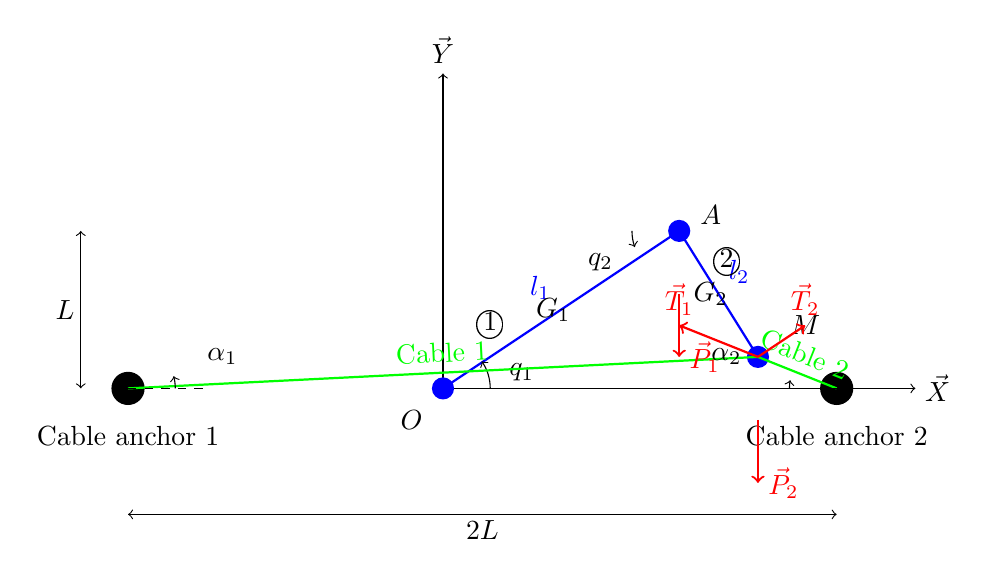
\begin{tikzpicture}[scale=2]
    % Coordinate system
    \draw[->] (0,0) -- (3,0) node[right] {$\vec{X}$};
    \draw[->] (0,0) -- (0,2) node[above] {$\vec{Y}$};
    \node at (-0.2,-0.2) {$O$};
    
    % Fixed base points
    \fill[black] (-2,0) circle (3pt);
    \fill[black] (2.5,0) circle (3pt);
    \node at (-2,-0.3) {Cable anchor 1};
    \node at (2.5,-0.3) {Cable anchor 2};
    
    % Serial arm links
    \draw[thick, blue] (0,0) -- (1.5,1) node[midway, above left] {$l_1$};
    \draw[thick, blue] (1.5,1) -- (2,0.2) node[midway, above right] {$l_2$};
    
    % Joints
    \fill[blue] (0,0) circle (2pt);
    \fill[blue] (1.5,1) circle (2pt);
    \fill[blue] (2,0.2) circle (2pt);
    
    % Joint labels
    \node at (0.3,0.4) {\textcircled{1}};
    \node at (1.8,0.8) {\textcircled{2}};
    \node at (2.3,0.4) {$M$};
    
    % Joint angles
    \draw[->] (0.3,0) arc (0:35:0.3);
    \node at (0.5,0.1) {$q_1$};
    \draw[->] (1.2,1) arc (180:200:0.3);
    \node at (1.0,0.8) {$q_2$};
    
    % Cable lines (both connected to end-effector M)
    \draw[green, thick] (-2,0) -- (2,0.2) node[midway, above, sloped] {Cable 1};
    \draw[green, thick] (2.5,0) -- (2,0.2) node[midway, above, sloped] {Cable 2};
    
    % Cable angles
    \draw[dashed] (-2,0) -- (-1.5,0);
    \draw[->] (-1.7,0) arc (0:15:0.3);
    \node at (-1.4,0.2) {$\alpha_1$};
    
    \draw[dashed] (2.5,0) -- (2,0);
    \draw[->] (2.2,0) arc (180:170:0.3);
    \node at (1.8,0.2) {$\alpha_2$};
    
    % Forces and positions
    \draw[->, red, thick] (1.5,0.6) -- (1.5,0.2) node[right] {$\vec{P}_1$};
    \draw[->, red, thick] (2,-0.2) -- (2,-0.6) node[right] {$\vec{P}_2$};
    
    % Cable tensions (both acting on point M)
    \draw[->, red, thick] (2,0.2) -- (1.5,0.4) node[above] {$\vec{T}_1$};
    \draw[->, red, thick] (2,0.2) -- (2.3,0.4) node[above] {$\vec{T}_2$};
    
    % Dimensions
    \draw[<->] (-2,-0.8) -- (2.5,-0.8);
    \node at (0.25,-0.9) {$2L$};
    \draw[<->] (-2.3,0) -- (-2.3,1);
    \node at (-2.4,0.5) {$L$};
    
    % Points G1, G2, A
    \node at (0.7,0.5) {$G_1$};
    \node at (1.7,0.6) {$G_2$};
    \node at (1.7,1.1) {$A$};
\end{tikzpicture}